% !TeX root = ../main.tex
% Add the above to each chapter to make compiling the PDF easier in some editors.

\chapter{Background and Related Work}\label{chapter:background}
This chapter briefly introduces the related topics of this thesis. The main topics are streaming, \gls{vr} and \gls{sr}.

\section{Streaming}\label{section:background_streaming}
Streaming includes technology that transmits video sequences over the Internet \parencite{Mok2011}. Today, streaming is a billion-dollar business dominated by global players like Amazon and Netflix \parencite{AMR2019} Moreover, for live events in sports, eSport and more, streaming is becoming essential \parencite{AMR2019}. Viewing television online is also becoming increasingly more popular as cable TV is becoming less common \parencite{CableTV}. 
\par
The technical aspects of streaming include multiple steps. For streaming normal movies or series, the data is encoded into a specific format or multiple formats independent of the user’s device, as each device can handles different codecs. For example Android can handle encoding and decoding H.263 up to H.265, VP8 and VP9, wheres AV1 can only be decoded and only on Smartphones having the Android 10 or greater \parencite{Android2020}. Some codecs were mentioned before, like the H.265 or VP9. Although the codecs differ in how they compute the compression and decompression, they have commonalities. For example, the different types of frames exist to deliver the best possible image. The intra-coded frame (I-frame) is a complete image. The predicted frame (P-frame) contains changes between the I-frames. When there are moving objects in a scene with a static background, only the moving object has to be encoded to save bandwidth. The third and last type is the bidirectional predictive frame (B-frame), which saves more bandwidth by calculating the difference by future, current and past frames \parencite{Katto1995}. The computation of these different types is called encoding. After the encoding, the video is transmitted through a network to the user’s device, where the different frames are merged, which is called decoding. Most modern hardware supports the decoding. Otherwise, a software decoder is required, which is less efficient than the hardware. The encoding and decoding are necessary to achieve an acceptable quality of the video. The lower or more unstable that the connection from the server to the client is, the higher the computation. Since users want stable, high-quality streaming, considerable efforts are required to meet this demand. For a stream having resolution below 720p, is non-stop buffering or is pixelated is not accepted by the user \parencite{VideoAcceptance}. Most video providers perform pre-encoding of the videos in different resolutions and codecs to be used by different kinds of user devices. Pre-encoding saves computation time, resources and money, because performing the videos’ analysis and math beforehand reduces the hardware load at delivery as the encoding is performed once. Furthermore, no action by the user of the system is involved \parencite{Netflix2015}.
\par
However, low latency is vital for streaming live public events for viewers to see the action and react at an appropriate time and with other viewers simultaneously. Alternatively, the viewer cannot receive what the commentator has to say in a timely manner with respect to the streamed event. The created lag impacts the viewing experience negatively.
Additionally, live events from private persons are becoming more popular. With YouTube, Facebook and Twitch, some popular platforms provide a free possibility to interact with hundreds of viewers at the same time. Low latency is required not to lose the ov erview, as the presenter directly interacts with his audience.
\par
The difference between regular and live streaming is that the video of the former does not exist in advance. The video cannot pre-encoded. Performing the encoding on-demand leads to a higher overall transmission time. To reduce the delay, the B-frames or the P-frames are disabled, as their computation is challenging and needs time. The remaining I-frames are whole images, which leads to a high bandwidth \parencite{Katto1995}. Typically, the live streams are not shared directly between the broadcaster and the spectators. Instead, between these two entities is a streaming distributor with more bandwidth capabilities than normal users have at home. The broadcaster uploads his video stream to the distributor, which shares the stream with the broadcasters’ viewers, as the broadcasters bandwidth capacity is limited and cannot handle many viewers. Examples of streaming distributors include YouTube \parencite{Youtube} or Twitch \parencite{Twitch}, which offer a complete platform with a full-service package. Moreover, other business-oriented delivery networks such as \cite{Akamai2020} exist. When latency is critical, a one-to-one connection is necessary to avoid all possible disturbances.

\section{Virtual Reality}\label{section:background_virtualreality}
The idea behind \gls{vr} was created in 1965 by \citeauthor{Sutherland195} with the title 'The Ultimate Display'. However, the first system able to show a virtual scene was created in 1962 by \citeauthor{Heilig1962} and was called Sensorama. Many iterations later, \gls{vr} is becoming applicable and affordable for many developers and users. For example, IKEA allows its customers to create virtual kitchens to inspect how their new kitchen would look like \parencite{Ikea2020}. Furthermore, the car manufacturer Audi shows a potential new car with all its possible configurations in a manner that is as realistic as possible for customers to have a better feeling of how the new car appears \parencite{Audi2017}. Moreover, in the medical sector, \gls{vr} is used to relieve amputees' phantom pain by controlling a virtual body part. Performing the movements is done by recording the electrical signals of the damaged limb \parencite{Murray2007}. All \glspl{hmd} displaying the virtual reality consists of two small screens directly in front of the user's eyes. In front of these screens are fish-eye lenses to create a spherical panorama. Both screens show the same content. Different techniques are used to create a steroscopic effent. One of them is to slightly shift the content horizontally on each screen presenting a different view of the scene to each eye. Moreover, other depth cues such as parallax, where objects in the distance move slower than the objects close up. Also lenses are used , where barrel distortion provides an enourmous field of fiew (FOV). These methods lead to an immersive 3D feeling for the user. 
\par
Aside from the stereoscopic effect or the design of the graphics, other factors impact whether the user thinks the virtual environment is realistic. Tracking the motion of the headset is essential to cultivate an immersive feeling. When the user rotates their head or moves, visualising the motion is essential. For example if the user rotates its head by a certain angle, the virtual view should rotate by the same angle. Some papers mention 11 milliseconds latency between the motion and the image refresh. Otherwise, a lack of realism due to motion sickness exists \parencite{Kim2018}. This notion 'refers to the illusion that the scenario being depicted is actually occurring' \parencite{Slater2009}, which means that the user feels that what is happening is real.


\begin{figure*}[t]
    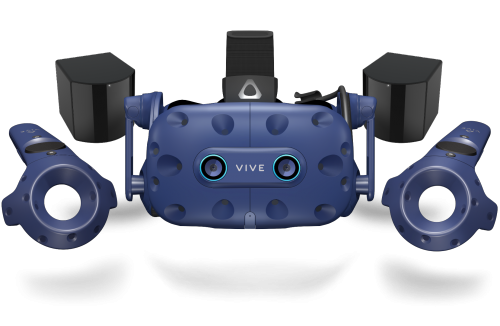
\includegraphics[width=\textwidth,height=\textheight,keepaspectratio]{logos/viveproeye.png}
     \caption{HTC VIVE Pro Eye, a \acrshort{vr} headset with controllers and tracking, image taken from \cite{HTCVIVEProEye2020}}
    \label{fig:htcviveproeye}
\end{figure*}

\section{Foveated Rendering}\label{section:background_foveatedrendering}

Foveated rendering is a new method of reducing the workload required for \gls{vr}. It was first mentioned in 2014 by FOVE, who invented the first head-mounted display with integrated eye-tracking to calculate foveated images based on the current gaze. With foveated rendering, the workload is lessened by reducing the image quality outside of the foveal area. As mentioned before, the foveal region is one of two regions of humans' vision. Foveated rendering recently reached consumer hardware, in particular through the VIVE Eye Pro \parencite{HTCVIVEProEye2020}, whereas a competitor, namely the Oculus Quest \parencite{Quest2020} supports a low-level implementation of foveated rendering called \gls{ffr} because of the lack of eye-tracking. \glsfirst{ffr} assumes a gaze more or less in the centre of the image. The developers set the hardness of the reduced quality in different steps. Foveated rendering's purpose is to reduce the number of pixels within the peripheral area. During runtime, the image is filled with interpolated pixels to achieve the desired size. Aside from reducing the workload by decreasing the calculated amount of pixels, foveated rendering also reduces the needed bandwidth as the image's size is reduced. To return the image to its original size, using \gls{sr} is an acceptable method.
\par
Foveated rendering is not only used for \gls{vr} gaming to lower the hardware. \citeauthor{Illahi2020} describe a method of how foveated rendering is also suitable for cloud gaming. In cloud gaming, the game is rendered through a server and streamed to the user. Simultaneously, the users' input is sent to the server so that on any device any game is playable independent of the users' hardware. In the paper by \citeauthor{Illahi2020}, the gaze is used for calculating a custom discrete cosine transformation (DCT) for the H.264 codec. In this codec, the image consists of pixel partitions from 16x16 to 2x2, but 8x8 blocks are primarily used. The block is processed by the DCT followed by a quantisation which requires a quantisation step \(Q_{step}\), which is precalculated and is applicable for all dimensions that are divided by eight. The paper proposes an offset for this \(Q_{step}\) bases on the current gaze, resulting in a foveated rendering where the more distant parts are more quantised and therefore have lower quality. 
\par
Furthermore, \citeauthor{Guenter2016} discuss how 360$^{\circ}$ videos are streamed with the technique of foveated rendering. They propose dividing an image into tiles and having smaller horizontal regions at the top and bottom and larger tiles in the middle as they are more in the users' view. Streaming each tile in low-resolution separately results in low bandwidth and reduces the computational need. The exception is when the tile is active, such as when the user actively looks into this tile, and then the tile is streamed in high-resolution. This technique allows efficient streaming of 360$^{\circ}$ videos without losing details, and having a sharp image in the users' gaze. 


\section{Superresolution}\label{section:background_superresolution}
A variety of image enhancement tools exist, including professional software like Adobe Photoshop \parencite{Adobe2020} as well as open-source projects like GIMP \parencite{Gimp2020}. These tools allow manual adjustments for better details, contrast and more. They also include tools to enhance a full image, for example deblurring a photo with the Wiener Filter \parencite{Wiener1964}. Using these tools requires experience, because blurring or other quality-weakening details need to be detected. For this reason, researching automatic image enhancements has become of interest to users, and new applications like video stream enhancements have become possible. One of them is \gls{sr}, which increases the size as well as enhances the quality.
\par
\Acrlong{sr} is a modern technique to enhance images. Improving images is necessary for multiple reasons, such as increasing the size if an image has a smaller spatial resolution than it should have. Another scenario is to have more details at specific regions, for example for cancer detection in an MRI scan by zooming into one region \parencite{Chaudhari2018}. The most general case is to have a beautiful image. Thus, analysing incoming images to determine the best possible options is essential, because the exact degradation function, is unknown. This function stores the information about defects such as blur and noise. Low-quality images are improved to good quality, and enhancing the images with good quality leads to more details by estimating them where they are unknown. Moreover, \gls{sr} reduces noise and blur in many cases. Performing the \gls{sr} in real-time is also necessary for some applications, such as live streaming or gaming. Simple methods perform the upscaling by interpolating nearby pixels to increase the overall number of pixels. However, related to the increasing attention given to movies, films or other moving images as well as the interest in better image quality, the research in \gls{sr} is making considerable progress.
\begin{figure*}[htbp]
    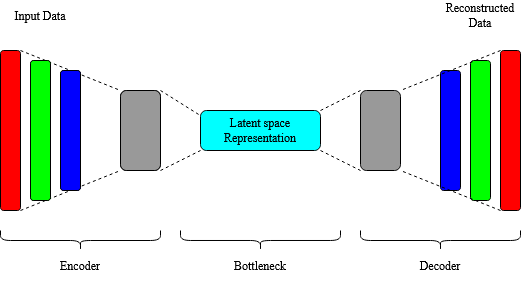
\includegraphics[width=\textwidth,height=\textheight,keepaspectratio]{logos/Autoencoder.png}
     \caption{Autoencoder}
    \label{fig:autoencoder}
\end{figure*}

\par
With \gls{dlss}, Nvidia launched one of the best-known \gls{sr} examples \parencite{DLSS2020}. It is capable of real-time \gls{sr} of 3D games. For this purpose, a deep convolutional neural network has an input of a low-resolution image as well as a motion vector which are both generated by the game engine. \gls{dlss} generates an image, which has a resolution one step higher. A step higher means that 540p input images have a 1080p or Full HD output image, whereas \gls{whqd} = 2560x1440 pixels images have a 4K resolution as an outcome. For their \gls{sr}, Nvidia used an architecture called convolutional autoencoder. The generated images were compared against 16K reference images, which resulted in a difference map which was forwarded back into the neural net to improve the results further. The remarkable aspect is that not every game is trained separately, as the network is trained generically and thus fits to a wide range of games. The original background of autoencoders is to learn efficient data representation. An autoencoder consists of an encoder making the data as dense as possible, most likely by dimensionality reduction. In \autoref{fig:autoencoder} the data has to be represented in such a manner that it fits through the bottleneck. On the other side of the bottleneck, there is a decoder with the goal to reconstruct the data by minimising the reconstruction error. Both the encoder and decoder are neural networks, typically with one hidden layer. Otherwise, the autoencoder is called deep autoencoder. There are the following two types of encoding:
\[x \neq d(e(x)) \]
whereas \(x\) represents the data, \(d(x)\) the decoding and \(e(x)\) the encoding.
The first equation represents the more probable situation, being the lossy encoding, where information is lost. In this subject, lossy means that the data cannot be fully restored after the compression. The other equation
\[x = d(e(x)) \]
represents the lossless encoding meaning that no data in the decoding is lost. As its only goal is to dense data, it is not capable of handling new data or even generating new data.

\par
\Acrlong{vae} where 'variational' comes from the variational inference, are one new step further and are capable of generating data. The \gls{vae} ensures that its latent space has good properties by regularising the distribution during training to generate new data. More specifically, it learns a latent variable model, which means it learns the parameters of a probability distribution which represents data instead of learning the data itself. It does not turn a sample into a parameter. Instead, it uses the mean \(\mu\) and the standard deviation \(\sigma\) of the data which are assumed. The stochastic encoding means that even for the same input, the actual encoding varies on every generation, which leads to a decoder having as input not only specific data points as generated by the standard autoencoder but also slightly varying encodings which cannot be differentiated. Thus, the \gls{vae} is capable of generating new data that looks similar to the existing material which can be generated randomly as well as in a specific direction. Additionally, as the range of \(\mu\) and \(\sigma\) are infinitely broad, the encoder has to learn these different values and ensure that it does not significantly vary from the same input. This behaviour allows the decoder to reconstruct the training data efficiently. Although the quality of the reconstruction and the desired outcome is dependent on the neural network that is used, it is a useful method for enhancing images. Variational autoencoders are one type of generative model, and another type are \glspl{gan}.

\begin{figure*}[htbp!]
    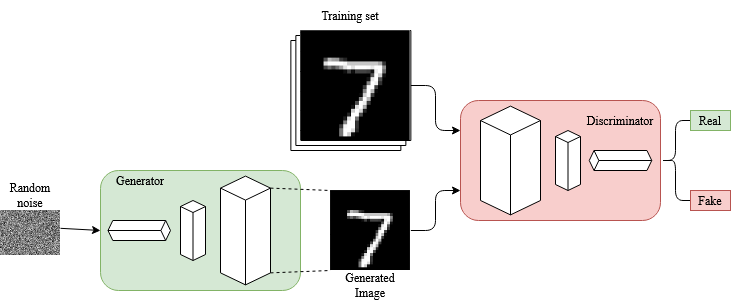
\includegraphics[width=\textwidth,height=\textheight,keepaspectratio]{logos/GANSchematic.png}
     \caption{Example of \acrshort{gan} as proposed by \cite{Goodfellow2014}}
    \label{fig:ganfigure}
\end{figure*}

\par
This type of neural network was initially developed to generate new images. It consists of two neural networks, a generator and a discriminator, that work against each other. The final goal is that a generator creates new images through random noise input. The training consists of the neural networks. The discriminator receives the images generated from both the generator and the training set as input and has to learn to differentiate them. The generator receives input of random noise as training and learns to generate images which look similar to the ones in the training set. The loss function of the generator is the result of the discriminator whether the image got accepted or not. An example of this outcome is presented in \autoref{fig:ganfigure}, where the well-known \gls{mnist} dataset is used \parencite{lecun2010}, which contains thousands of handwritten digits. In this example, the generator tries to generate a number which is accepted by the discriminator. Aside from having noise as the input, a further step is to use other images as input that contain small structures. Images of a semantic object can be used in Pix2Pix networks to generate a complete image of them, for example generating an image of a complete house from a drawn building \parencite{isola2018}. This process also permits characteristic features of images to be mixed, which is enabled by a CycleGAN where for example, adding the stripes of a zebra to a horse \parencite{zhu2020}. A CygleGAN enables to train neural networks to translate an image to a target domain without paired examples, i.e. the target image is newley created without an ideal image. Increasing a smaller image in size without losing details is difficult even for modern techniques. Another well-working example for \gls{sr} is the \glsfirst{srgan} proposed by \cite{Ledig2017} which is built upon a \gls{gan}. The goal of \gls{srgan} is to learn the statistics behind a high-resolution image of a training set and determine how to get there from the lower resolution image. In comparison to the \gls{vae}, the learning process is different, and in a \gls{gan} another neural network decides whether the generated image is satisfactory. As the generator and discriminator work against each other, an equilibrium between these two achieves the best results. Alternatively, \gls{vae} maximises the lower bound of the log-likelihood. Therefore, \gls{vae} is more comfortable to train, as training only one network is necessary, which is in contrast to the training of two networks with \gls{gan} and keeping them both equal. As an example, \autoref{fig:srexample} demonstrates the differences between the \gls{srgan} generated image, the low-resolution input and the original high-resolution image. However, the generator does not necessarily have to increase the image size, as the other implementations have shown.

\begin{figure*}[t]
    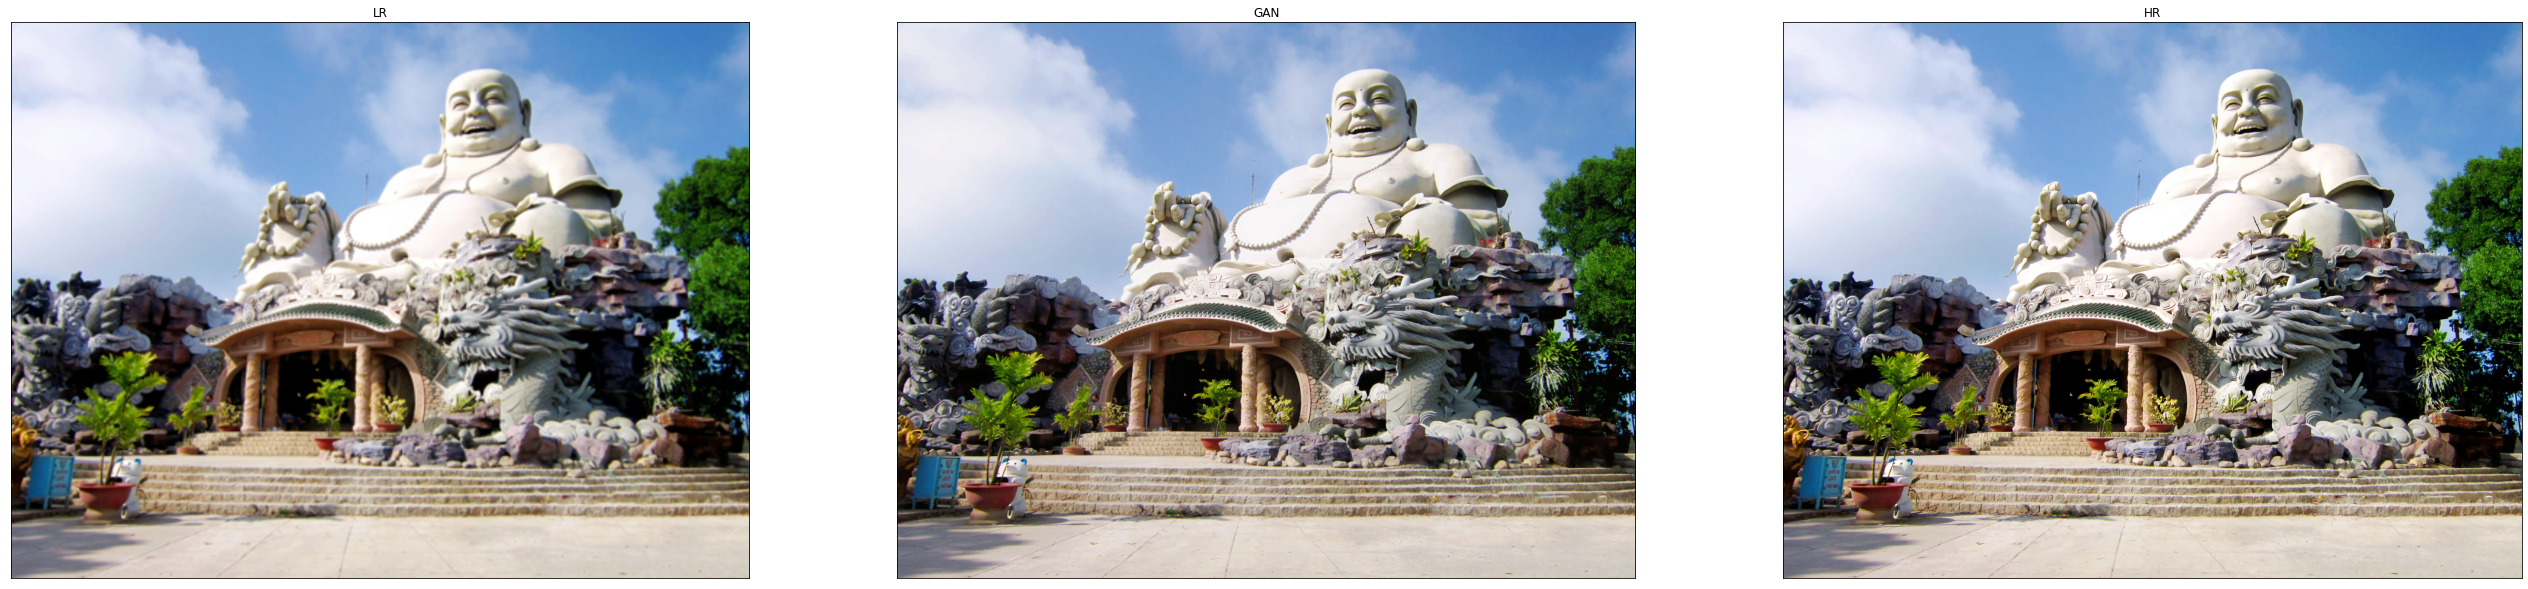
\includegraphics[width=\textwidth,height=\textheight,keepaspectratio]{logos/SR.png}
     \caption{Example of \gls{sr} as proposed by \cite{Ledig2017} with an example image from the DIVK dataset \parencite{Agustsson2017} }
    \label{fig:srexample}
\end{figure*}

\par	
In conclusion, multiple possibilities exist to generate new images out of existing images to add details, to compress them without losing details or to mix features. The presented two solutions namely the \gls{vae} and the \gls{gan} are the most promising ones as they achieve the best results. 

